\section{Introduction \& Background}

\subsection{General Introduction}
%%%%%%%%%%%%%%%%%%%%%%%%%%%%%%%%%%   1    %%%%%%%%%%%%%%%%%%%%%%%%%%%%%%% 
\begin{withoutheadline}
\begin{frame}{ General Introduction}


\setbeamercolor{block title}{bg=blue!30,fg=black}
\setbeamercolor{block body}{bg=blue!10,fg=black}
\setbeamertemplate{blocks}[rounded][shadow=false]

\begin{block}{ IoT \& Wireless Sensor Networks}
    \begin{itemize}
    \item Network technologies and IoT. 
    \item<2-> WSN: standardization of IoT nodes communication.
    \item<3-> Low power consumption, low cost.
    \item<4->  IEEE802.15.4 one of the main standards of WSN. 
    \end{itemize}
    \end{block}

 \begin{figure}[p]

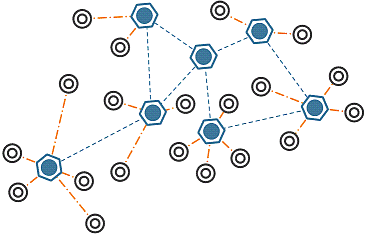
\includegraphics[width=0.5\linewidth]{figures/wsn.png}
  
\end{figure}

\end{frame}
\end{withoutheadline}
%%%%%%%%%%%%%%%%%%%%%%%%%%%%%%%%%%   2   %%%%%%%%%%%%%%%%%%%%%%%%%%%%%%%%

\begin{withoutheadline}
\begin{frame}{General intoduction}{IEEE802.15.4}

\setbeamercolor{block title}{bg=blue!30,fg=black}
\setbeamercolor{block body}{bg=blue!10,fg=black}
\setbeamertemplate{blocks}[rounded][shadow=false]


\begin{minipage}[t]{0.48\linewidth}

\begin{block}{Converge Cast Structure}
    \begin{itemize}
    \item Nodes radio ranges defines the neighborhood.
    \item<2-> \alert{Sink} is selected. 
    \item<3-> Packets are forwarded \alert{toward the sink}.
    \item<4-> Communication pairs.
    \end{itemize}
    \end{block}
\end{minipage}\hfill
\begin{minipage}[t]{0.48\linewidth}
\centering
 \begin{figure}[p]

 \only<1>{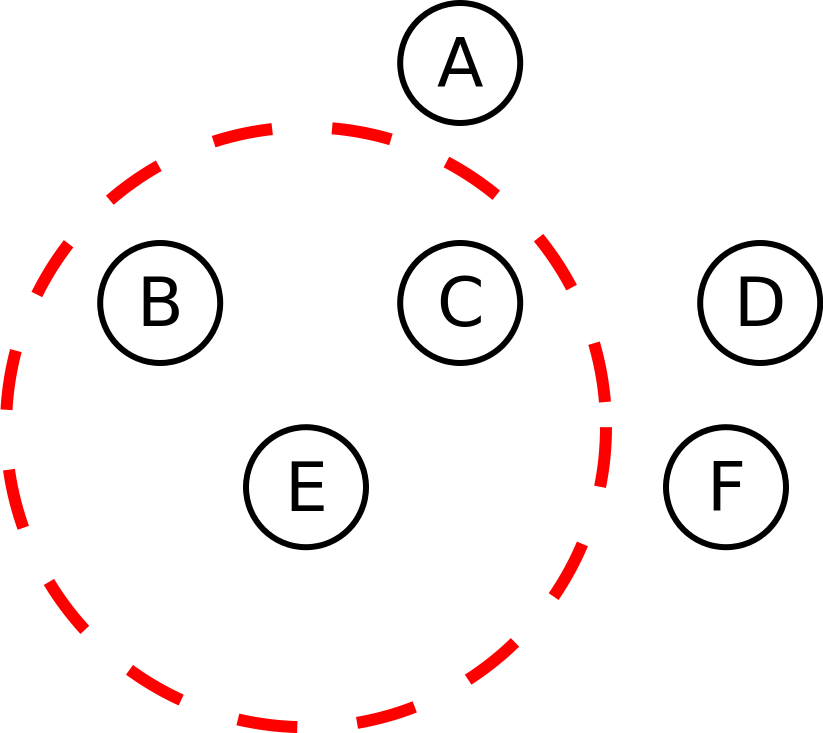
\includegraphics[width=\linewidth]{figures/map1.png}}
  \only<2>{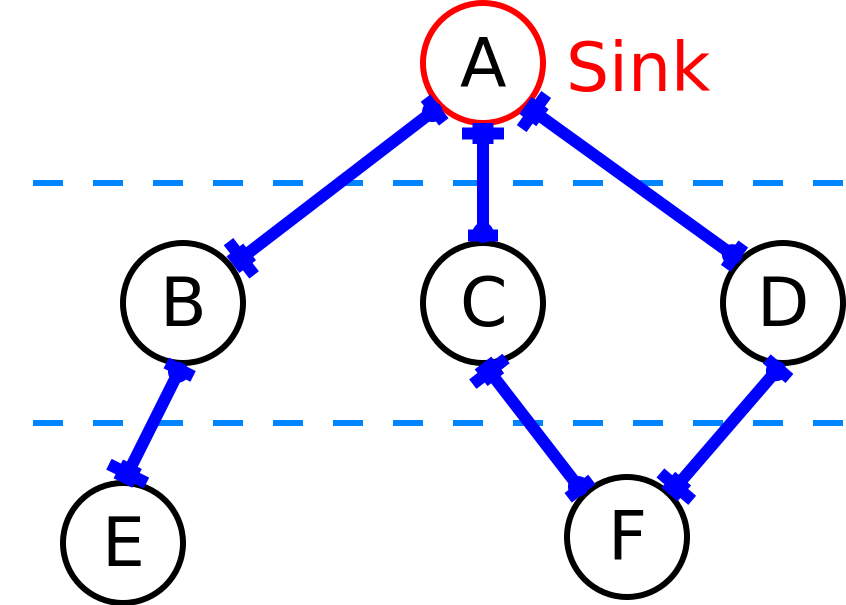
\includegraphics[width=\linewidth]{figures/map2.png}}
  \only<3>{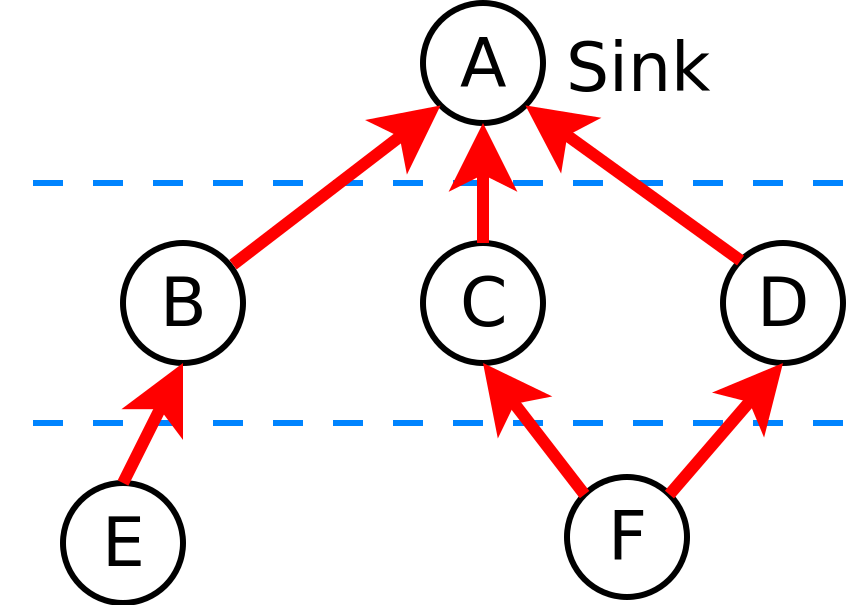
\includegraphics[width=\linewidth]{figures/map3.png}}
  \only<4>{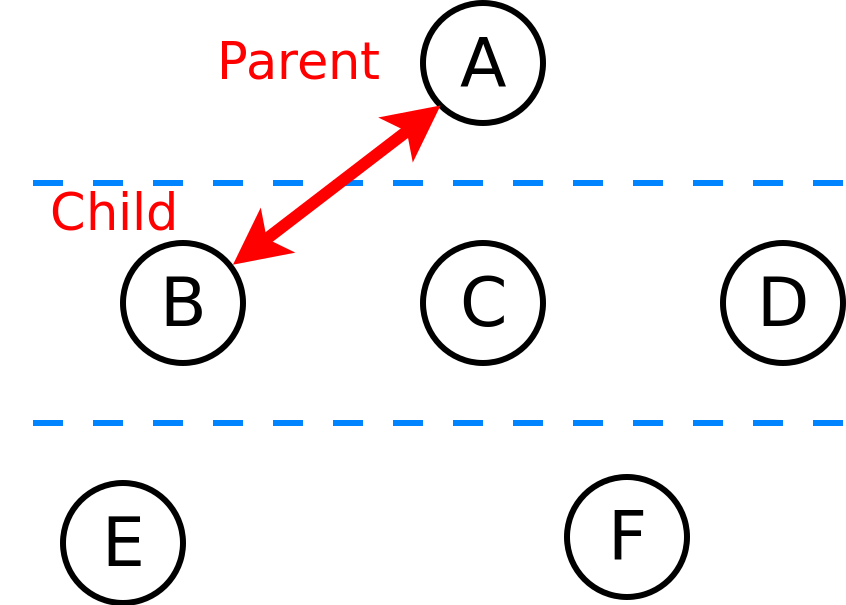
\includegraphics[width=\linewidth]{figures/map4.png}}
  
\end{figure}
\end{minipage}

   
    
    

\end{frame}
\end{withoutheadline}

%%%%%%%%%%%%%%%%%%%%%%%   IEEE802.15.4 Protocols  %%%%%%%%%%%%%%%%%%%%%%%
\subsection{IEEE802.15.4 Protocols}
%%%%%%%%%%%%%%%%%%%%%%%%%%%%%%%%%%   3   %%%%%%%%%%%%%%%%%%%%%%%%%%%%%%%%
\begin{withoutheadline}
\begin{frame}{IEEE802.15.4 Protocols}

\setbeamercolor{block title}{bg=blue!30,fg=black}
\setbeamercolor{block body}{bg=blue!10,fg=black}
\setbeamertemplate{blocks}[rounded][shadow=false]

\begin{block}{IEEE802.15.4e TSCH}
    \begin{itemize}
    \item  IEEE802.15.4 defines the MAC and PHY layers. 
    \item  TSCH is an extension of the MAC layer of IEEE802.15.4.
    \item<2->  Time/Frequency multiplexing of the bandwidth.
    \item<3-> Shared cells/Dedicated cells..
    \item<6-> 6TiSCH operation sublayer 6top will manage the TSCH.
    \end{itemize}
    \end{block}

\begin{figure}[p]

 \only<1>{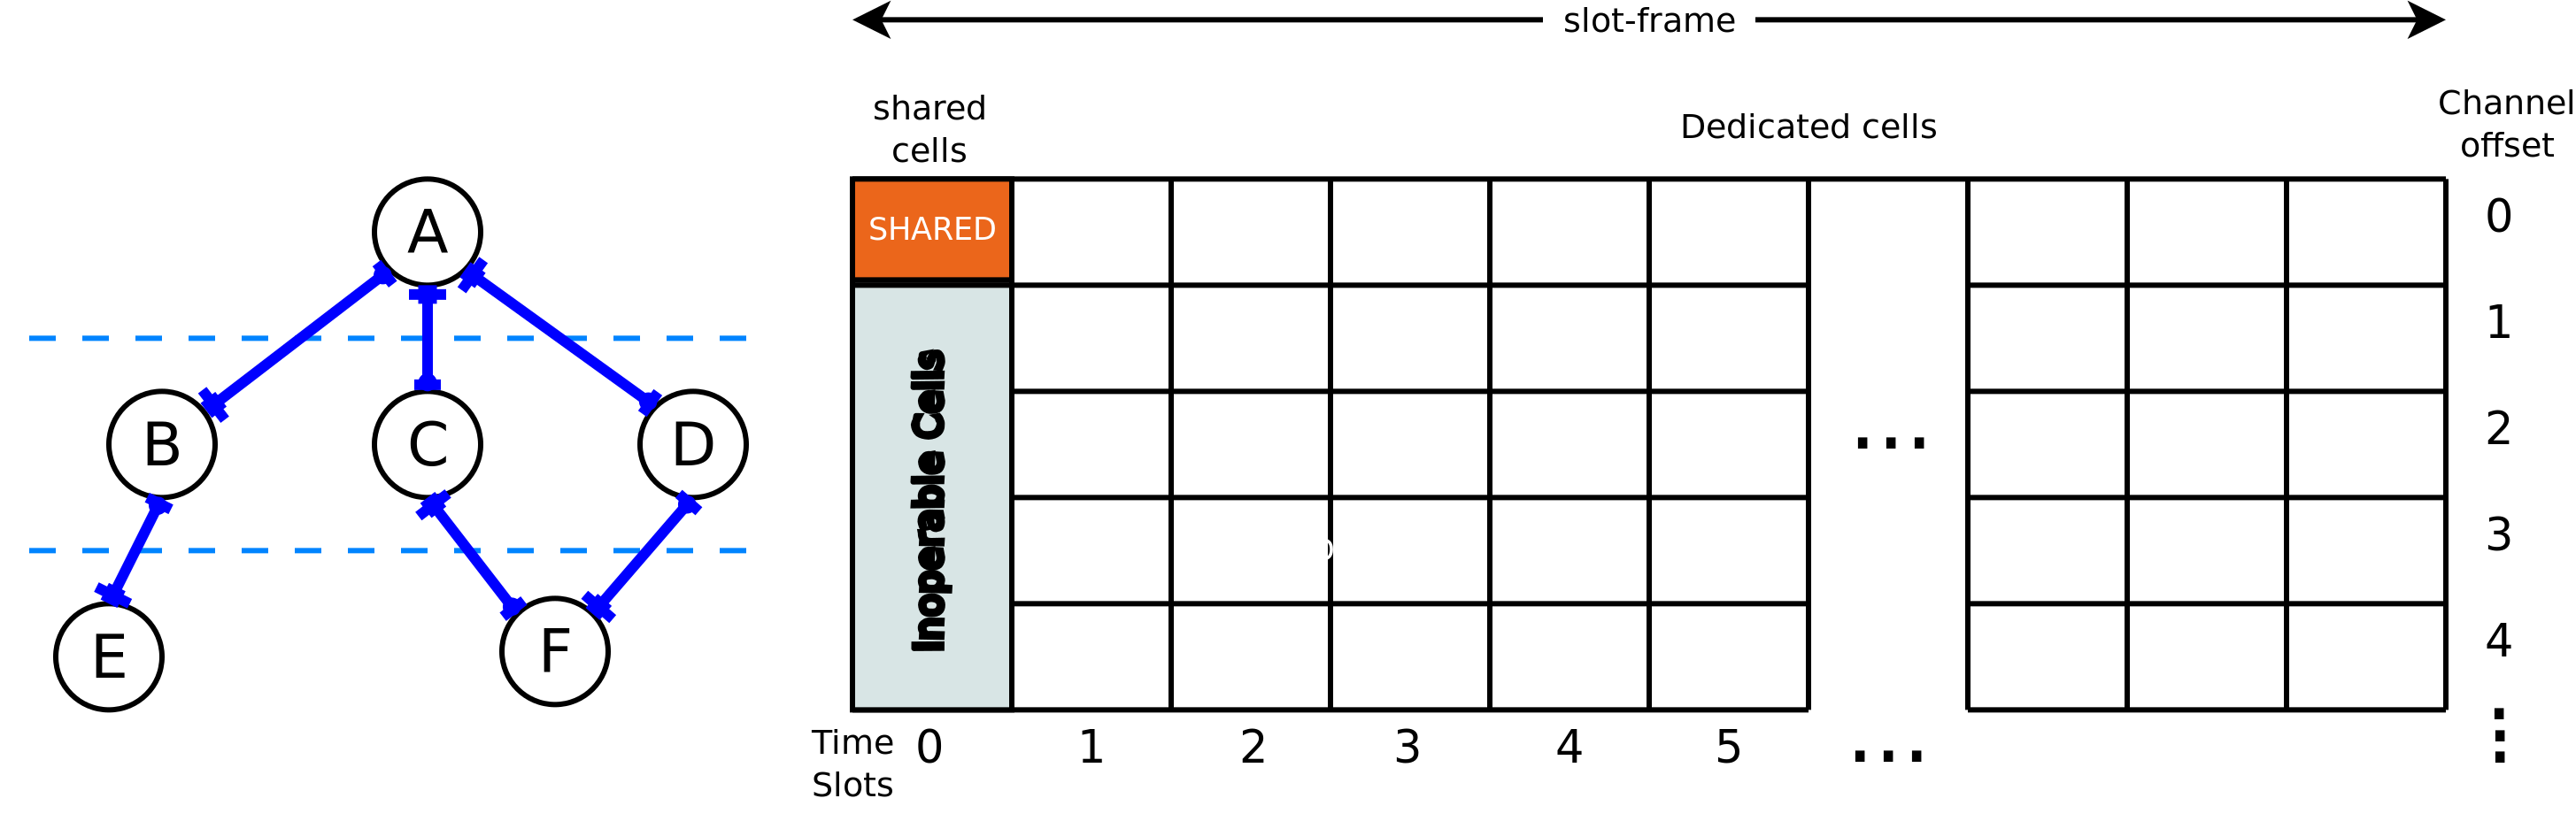
\includegraphics[width=\linewidth]{figures/TSCH1.png}}
  \only<2>{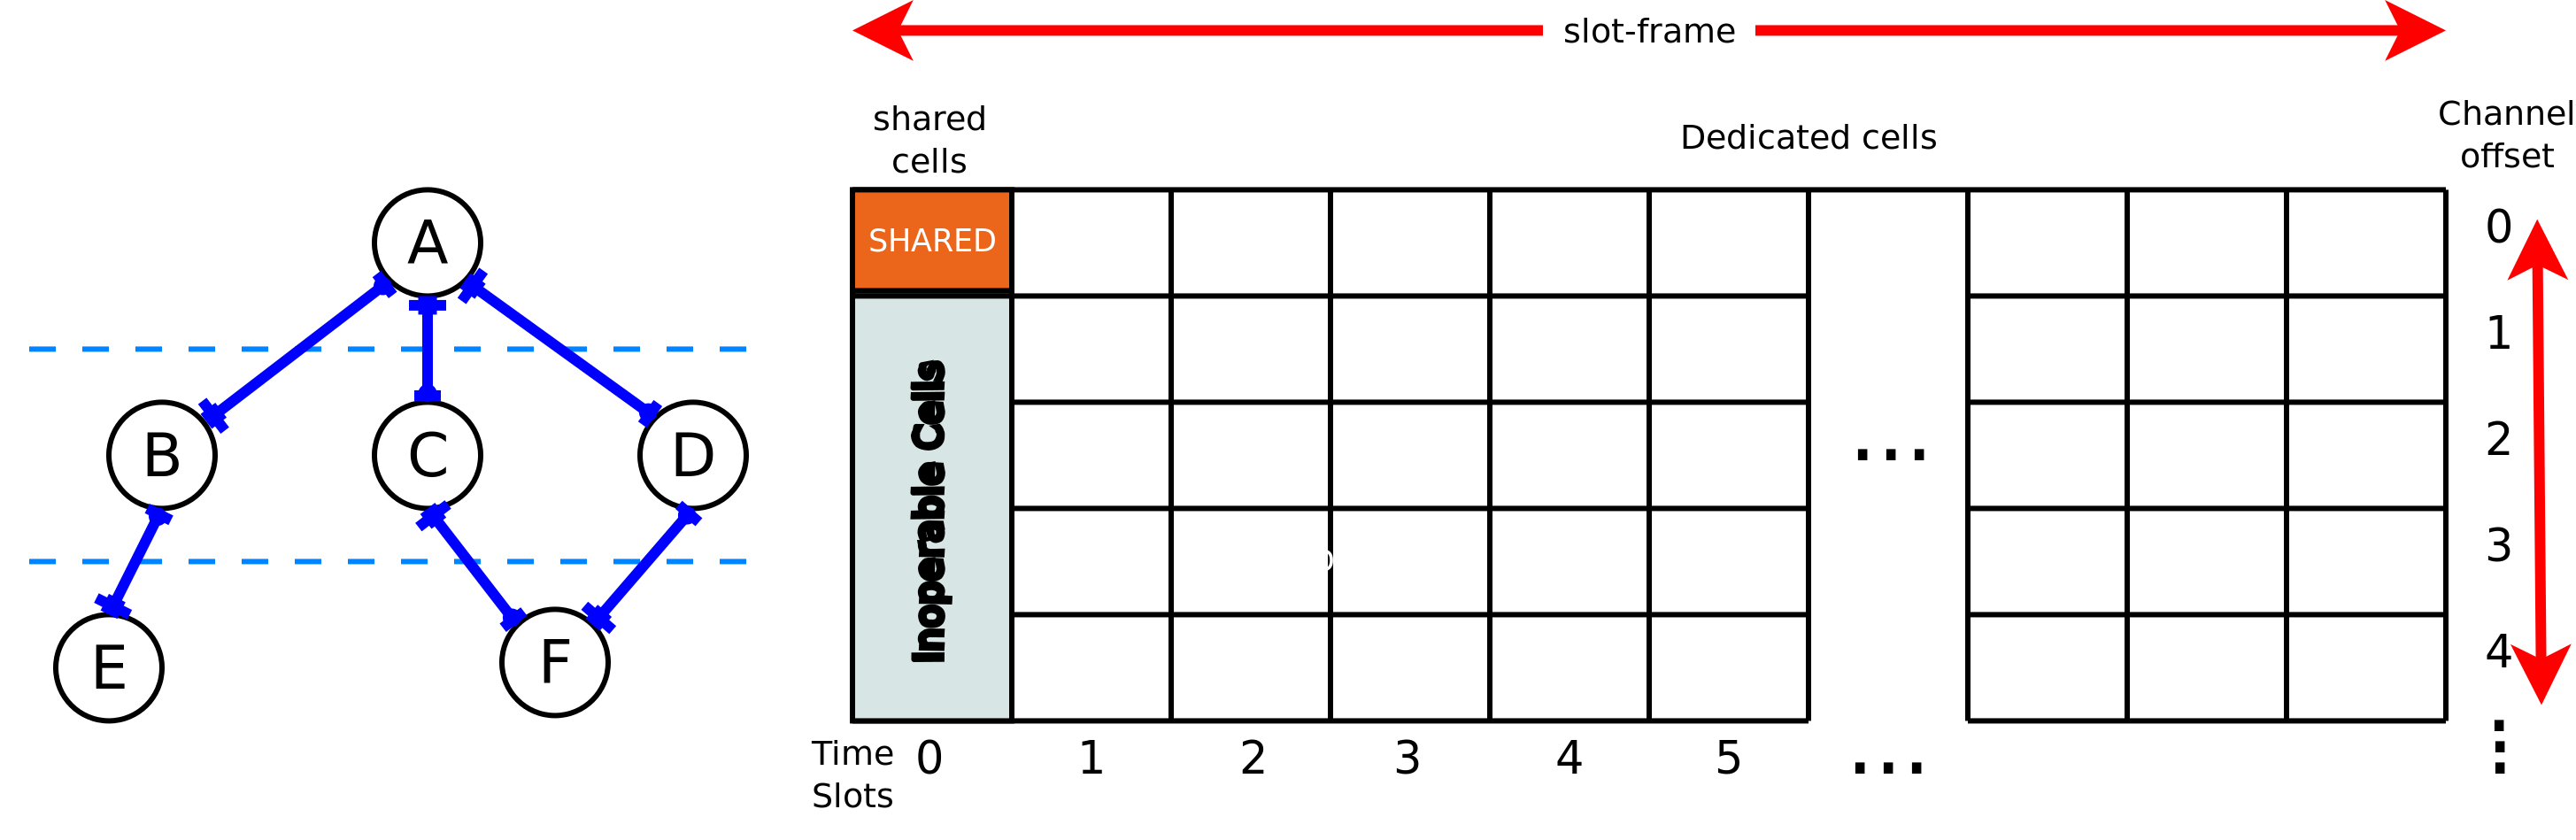
\includegraphics[width=\linewidth]{figures/TSCH2.png}}
  \only<3>{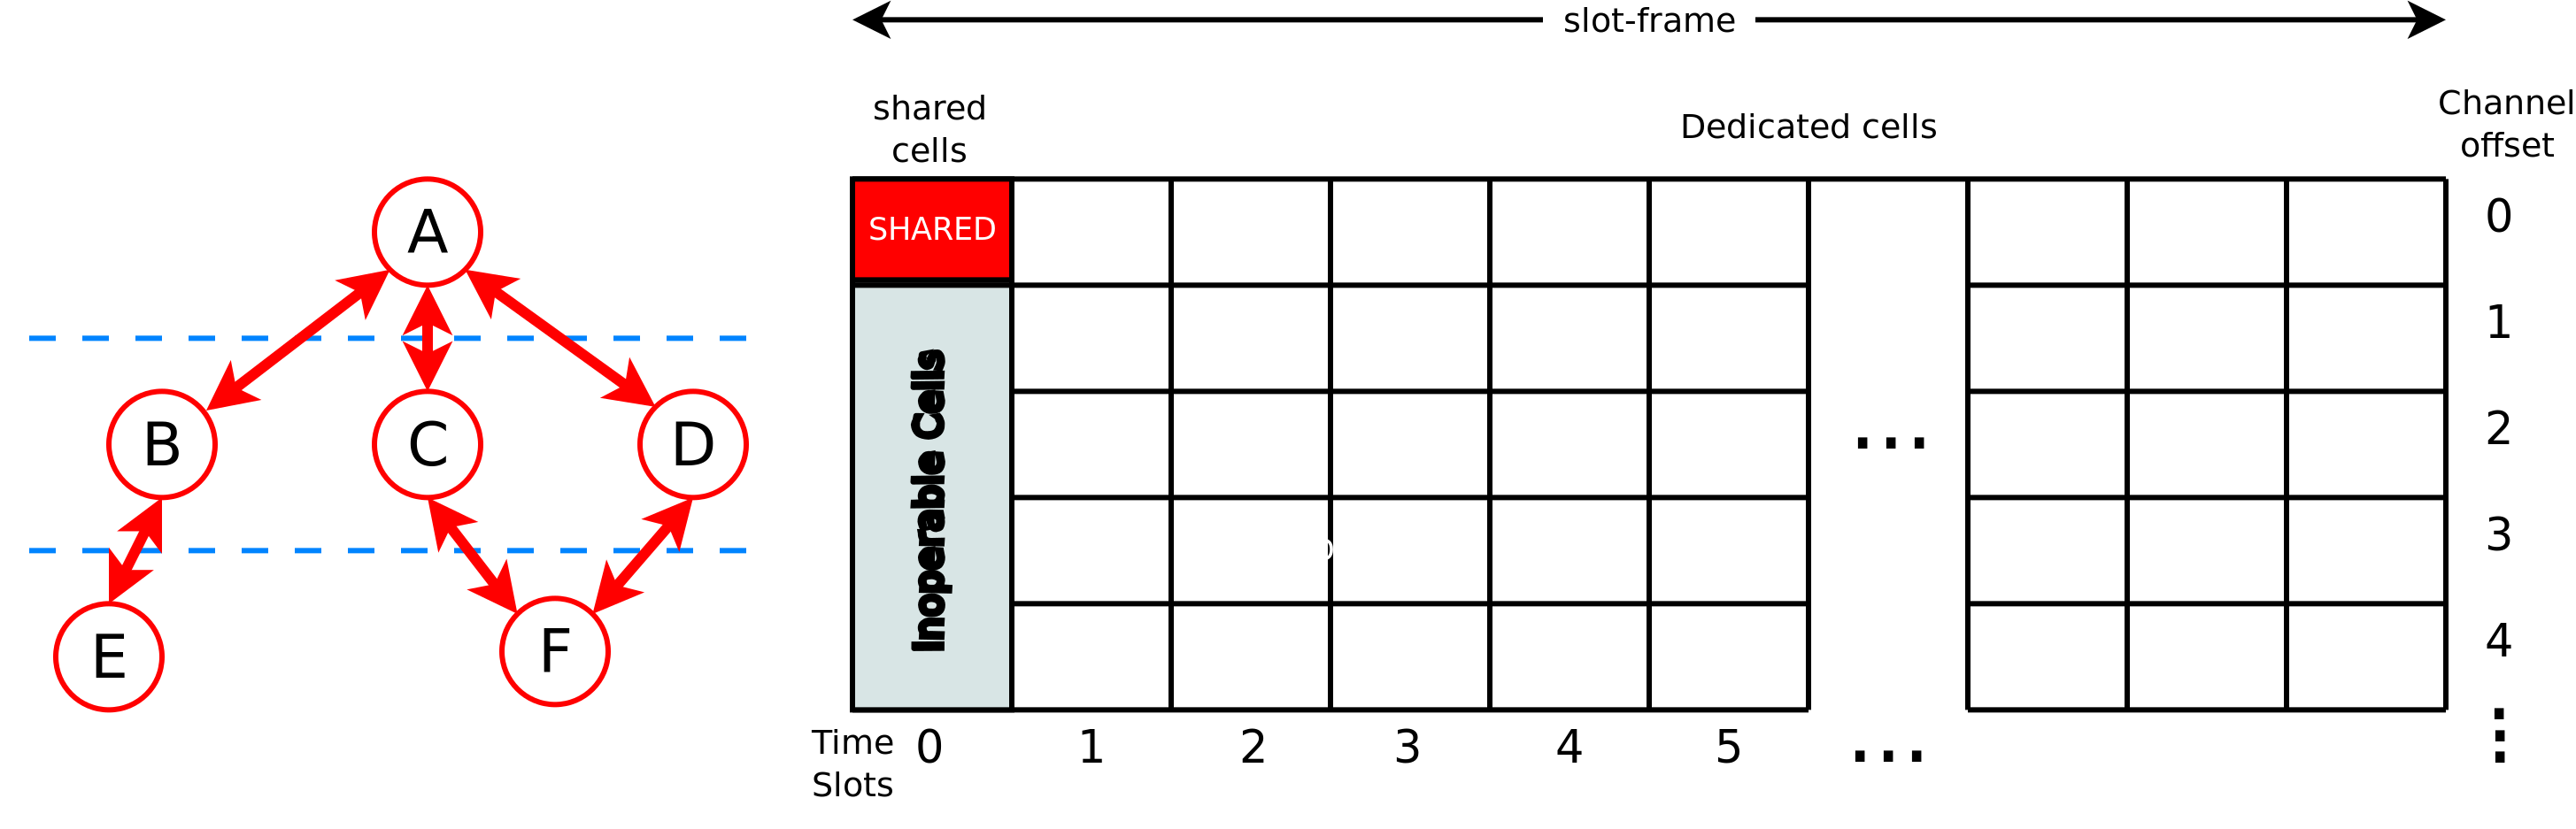
\includegraphics[width=\linewidth]{figures/TSCH3.png}}
      \only<5>{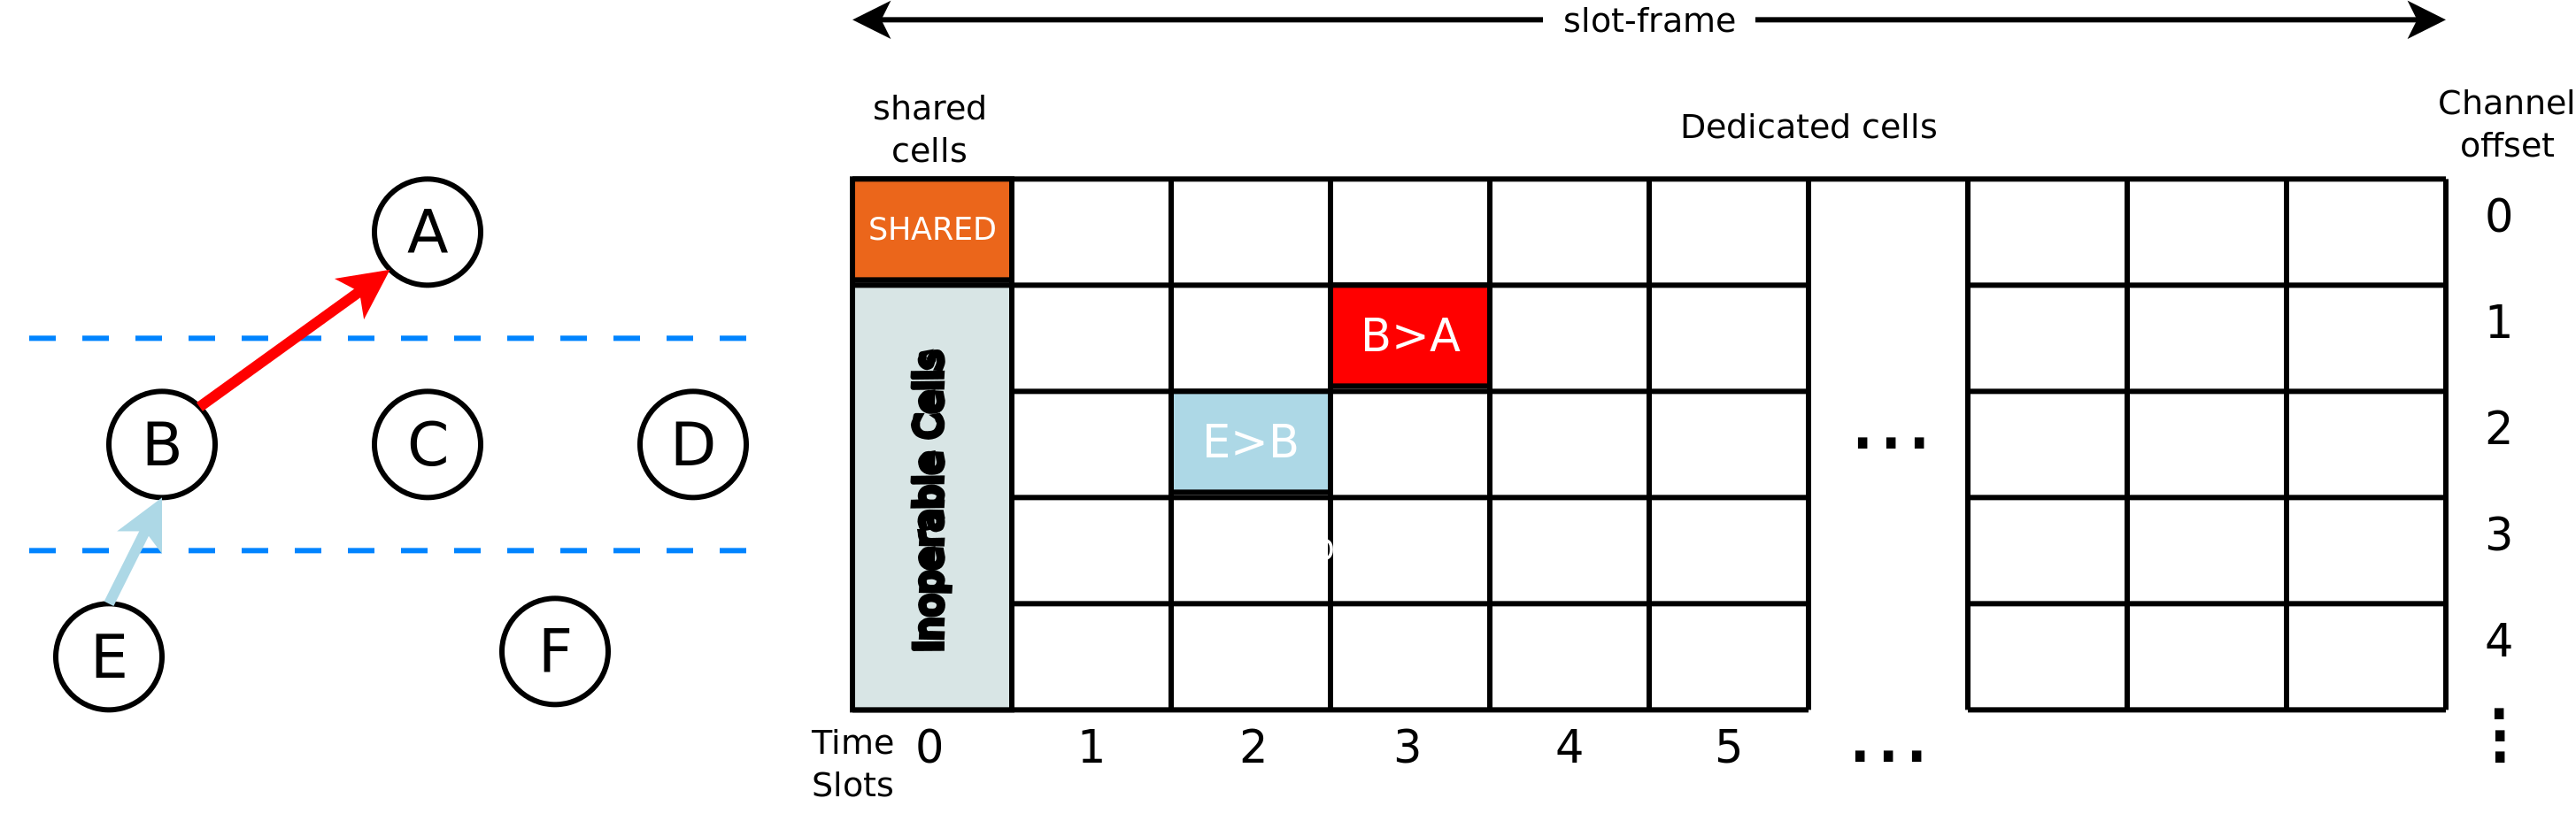
\includegraphics[width=\linewidth]{figures/TSCH5.png}}
\end{figure}


\end{frame}
\end{withoutheadline}
%%%%%%%%%%%%%%%%%%%%%%%%%%%%%%%%%%   4   %%%%%%%%%%%%%%%%%%%%%%%%%%%%%%%%


%%%%%%%%%%%%%%%%%%%%%%%%%%%%%%%%%%  5   %%%%%%%%%%%%%%%%%%%%%%%%%%%%%%%%
\begin{withoutheadline}
\begin{frame}{IEEE802.15.4 Protocols}


\setbeamercolor{block title}{bg=blue!30,fg=black}
\setbeamercolor{block body}{bg=blue!10,fg=black}
\setbeamertemplate{blocks}[rounded][shadow=false]
\begin{block}{Cell Reservation Process}
    \begin{enumerate}
    
    
    \item  Scheduling function decides new cell should be assigned.
    \item<2-> Child node sends an Add request. 
    \item<3-> Scheduling function decides which cells to be selected. 
    \item<4-> Parent node replies with an Add response.
    \item<5-> Cell is added and communication start.
    \end{enumerate}
    \end{block}

\begin{figure}[p]

 \only<1>{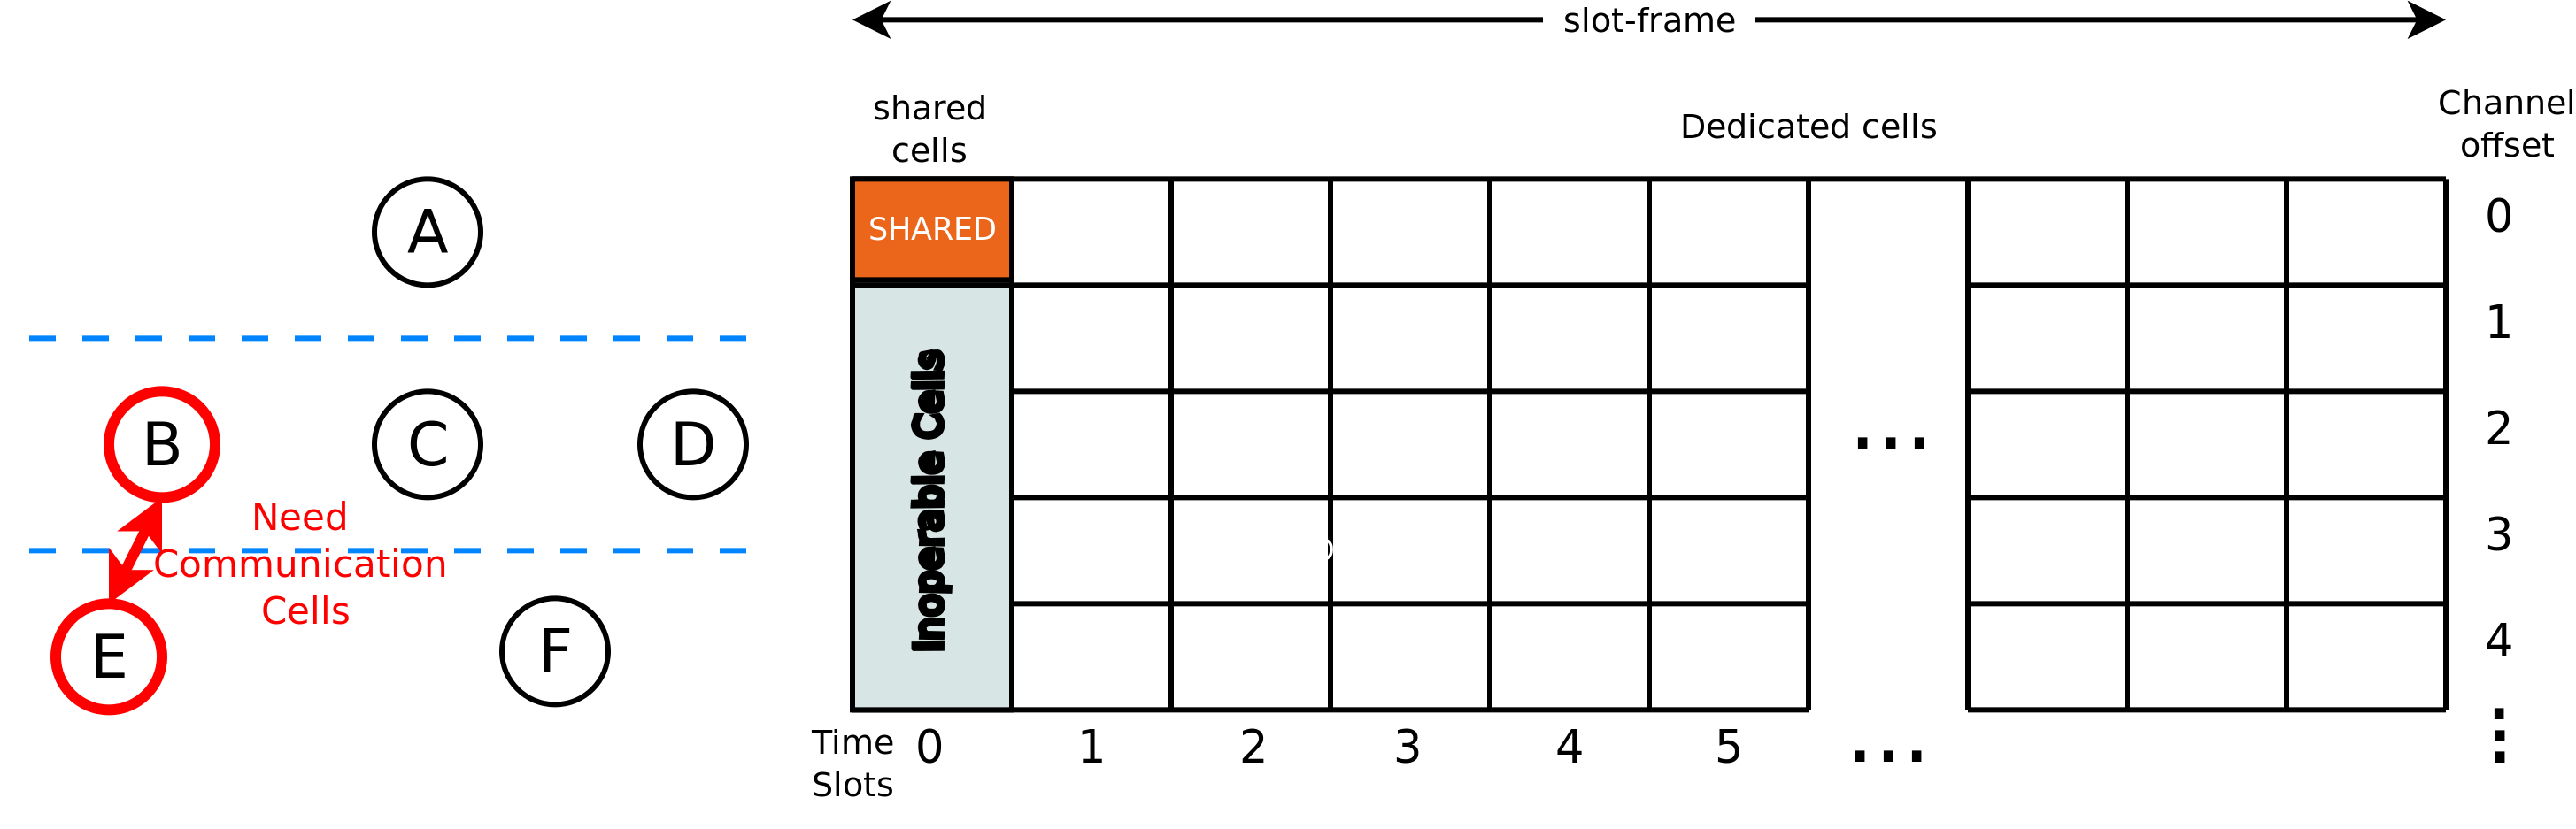
\includegraphics[width=\linewidth]{figures/6top1.png}}
  \only<2>{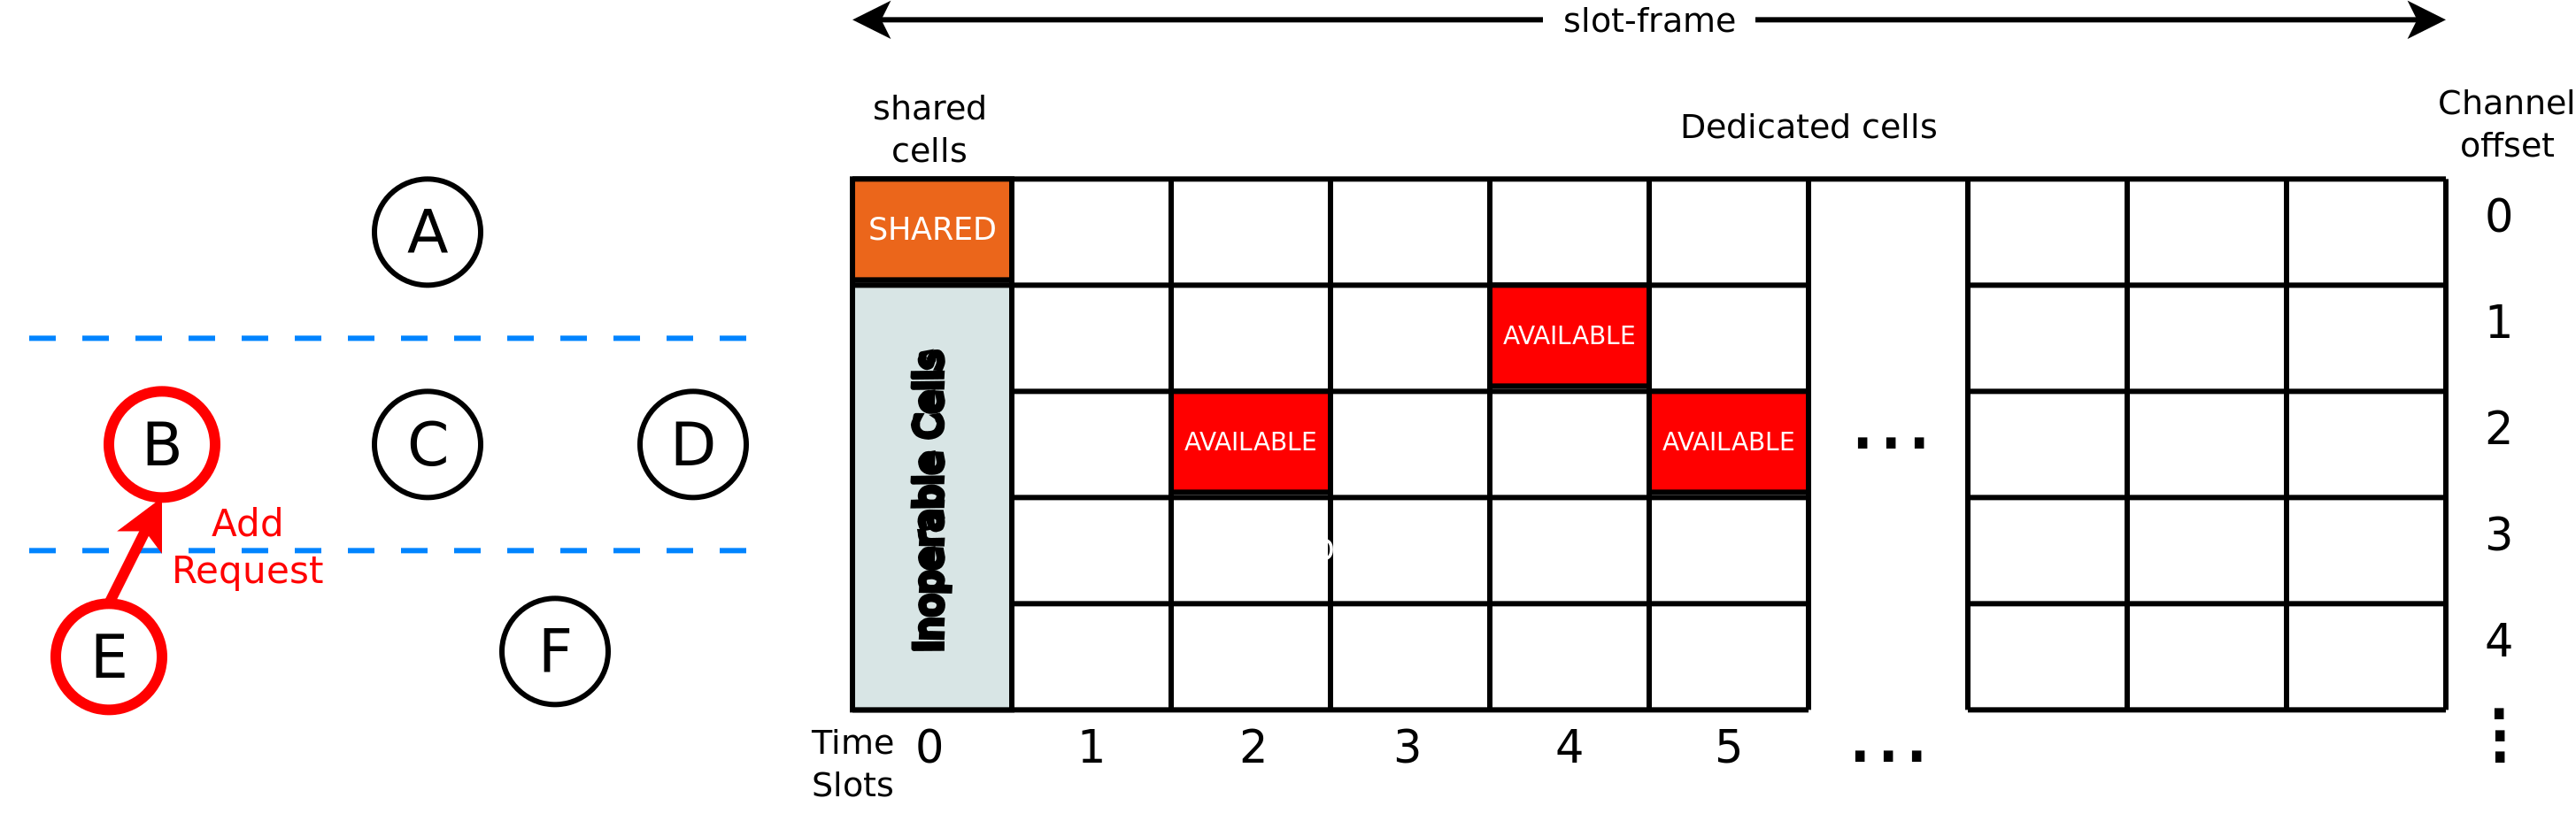
\includegraphics[width=\linewidth]{figures/6top2.png}}
  \only<3>{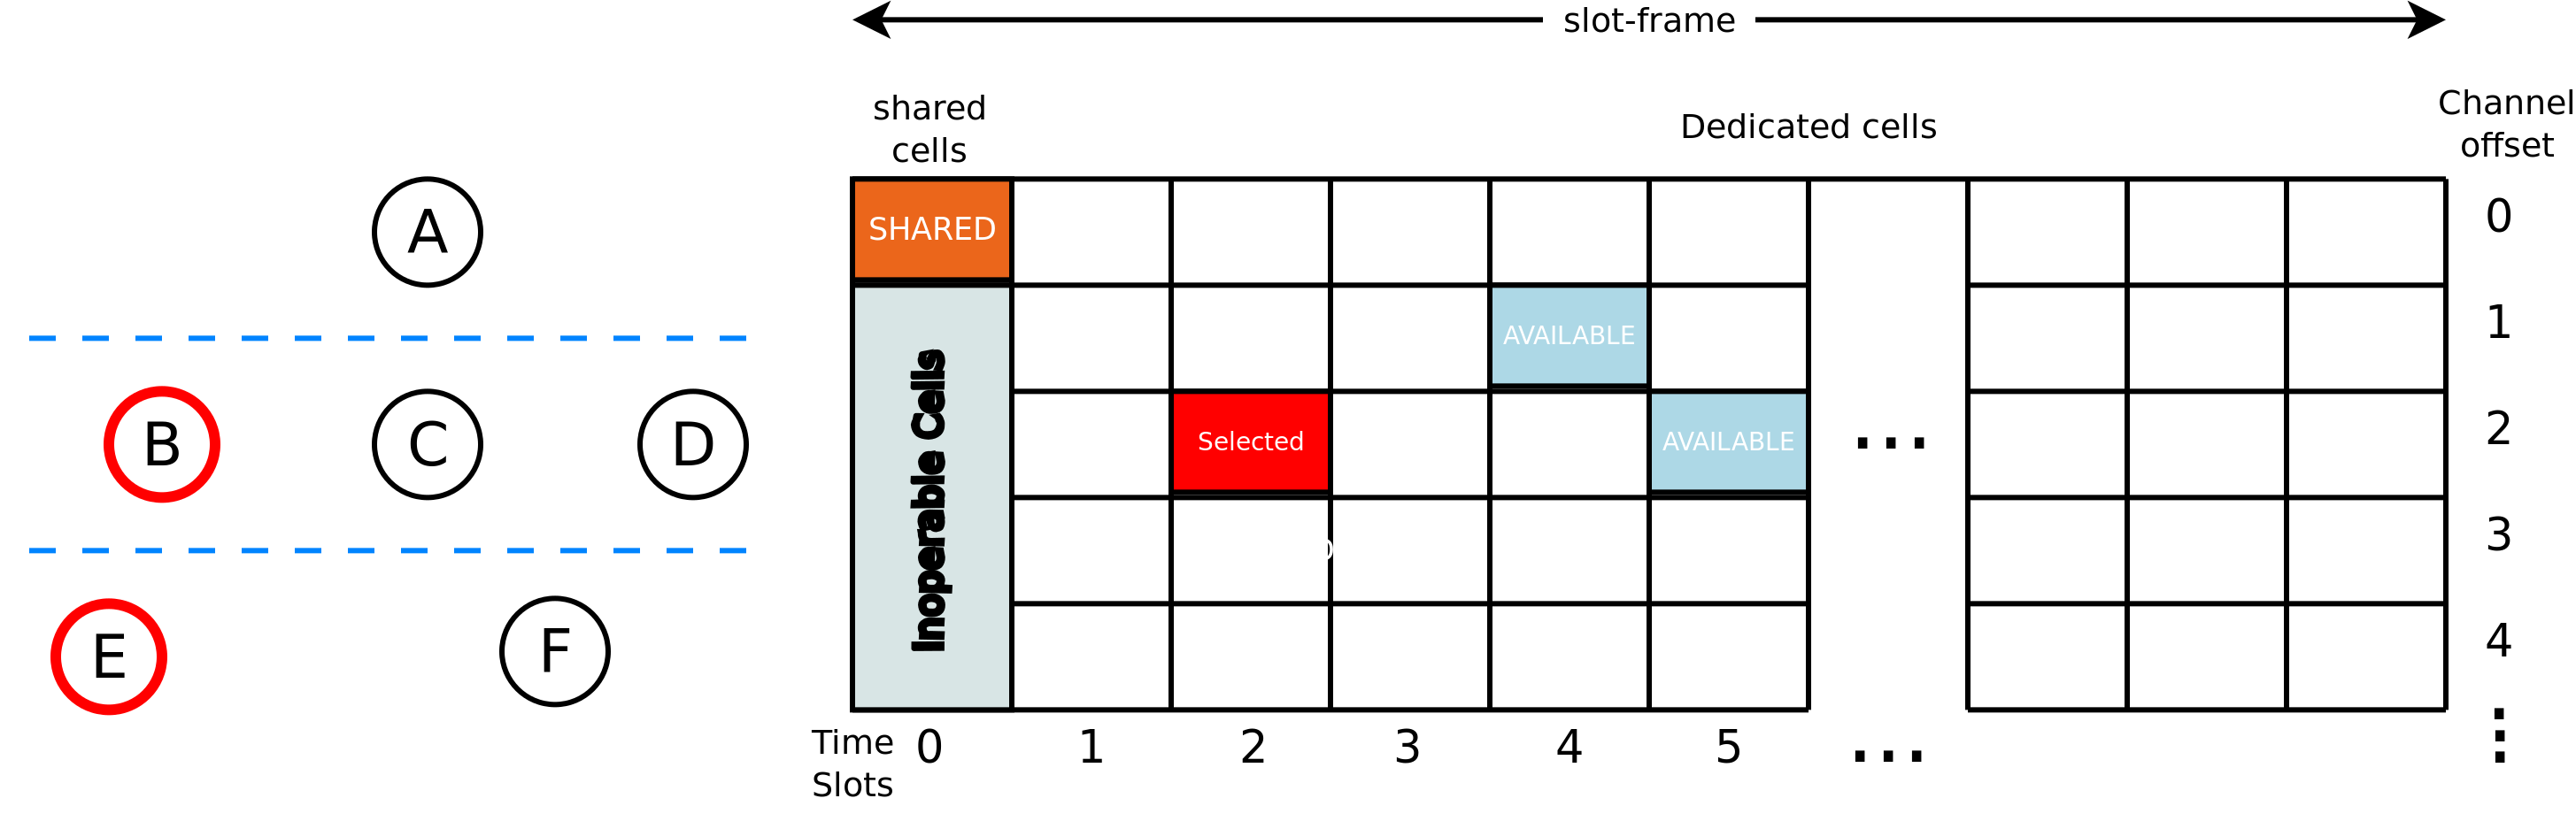
\includegraphics[width=\linewidth]{figures/6top3.png}}
  \only<4>{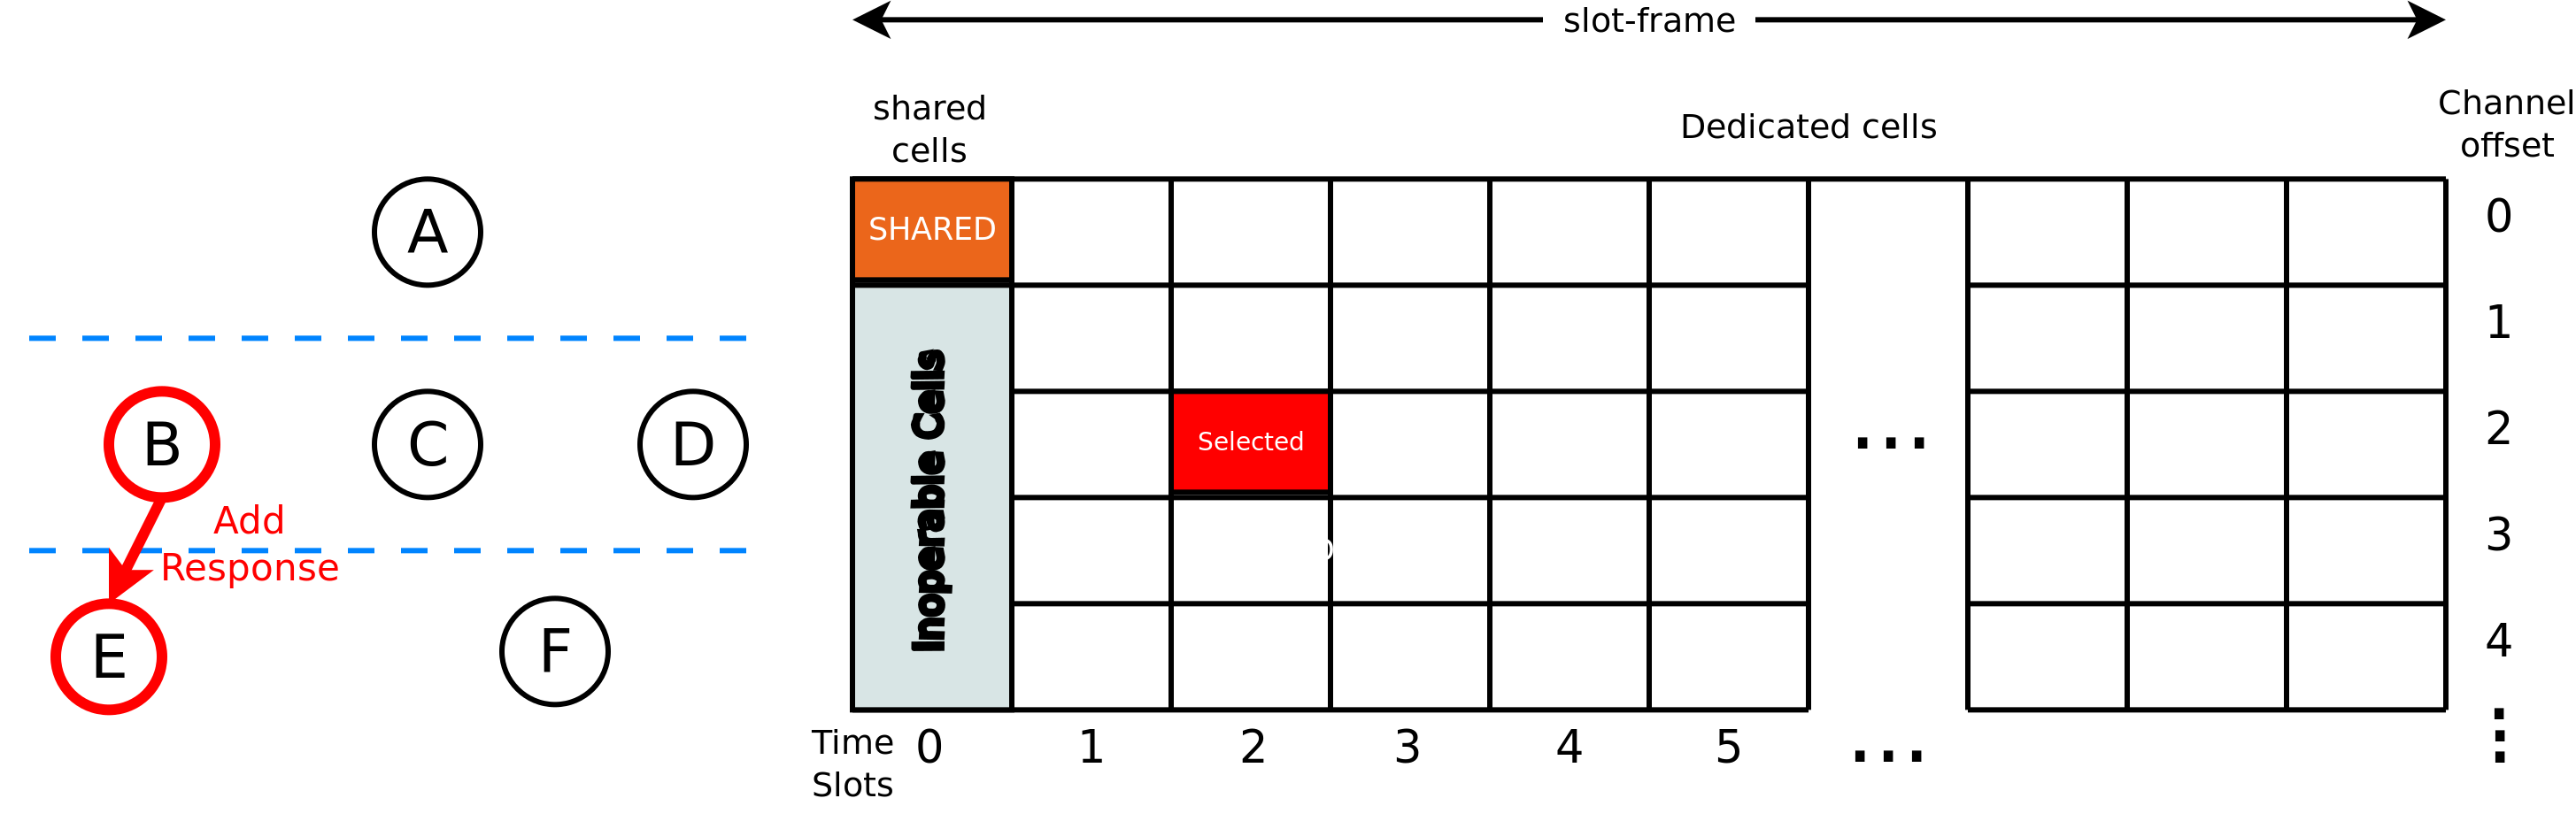
\includegraphics[width=\linewidth]{figures/6top4.png}}
    \only<5>{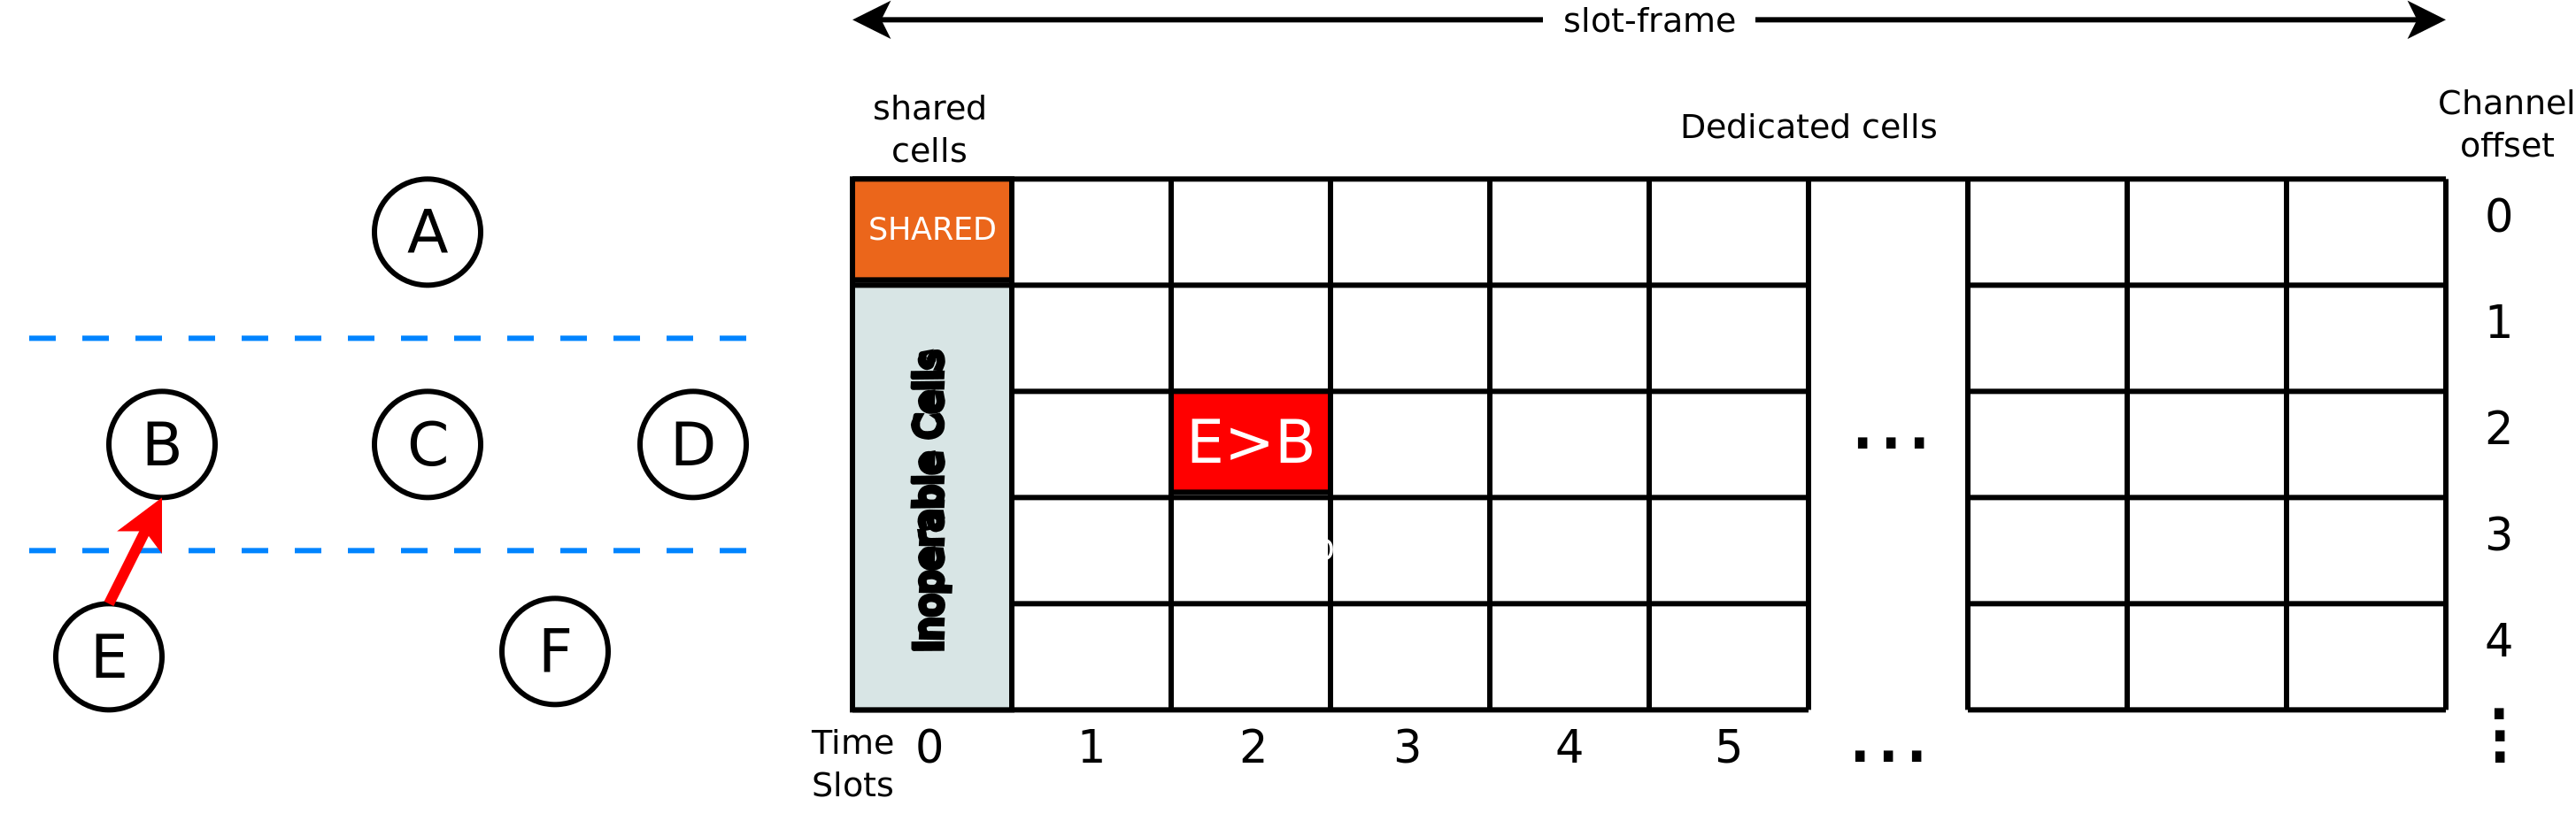
\includegraphics[width=\linewidth]{figures/6top5.png}}
\end{figure}




\end{frame}
\end{withoutheadline}

%%%%%%%%%%%%%%%%%%%%%%%%%%%%%%  Objectives  %%%%%%%%%%%%%%%%%%%%%%%%%%%%

\subsection{Project challenges \& Objectives}
%%%%%%%%%%%%%%%%%%%%%%%%%%%%%%%%%%  6   %%%%%%%%%%%%%%%%%%%%%%%%%%%%%%%%
\begin{withoutheadline}
\begin{frame}{Project challenges \& Objectives}


\setbeamercolor{block title}{bg=blue!30,fg=black}
\setbeamercolor{block body}{bg=blue!10,fg=black}
\setbeamertemplate{blocks}[rounded][shadow=false]

\begin{block}{Collision in Dedicated Cells}
    \begin{itemize}
    \item Collision free Dedicated Cells?  
    \item Neighbor nodes can select the same communication cell.
    \item<3-> Collision at the reception Node.
    
    \end{itemize}
    \end{block}

\begin{figure}[p]

 \only<1>{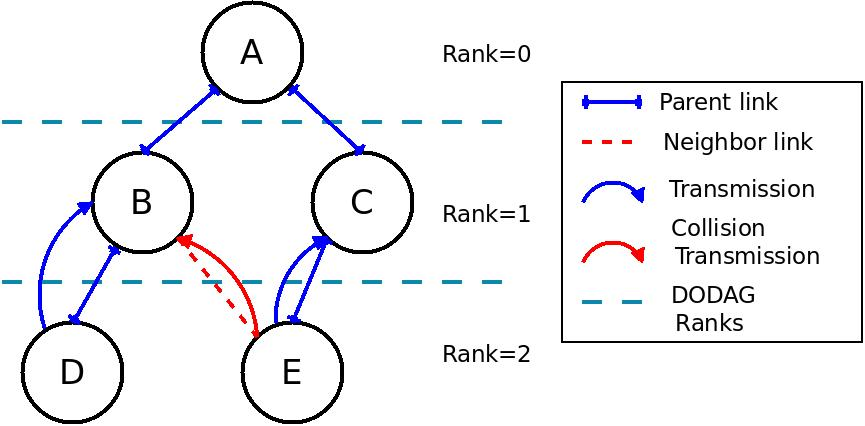
\includegraphics[width=\linewidth]{figures/col1.png}}
  \only<2>{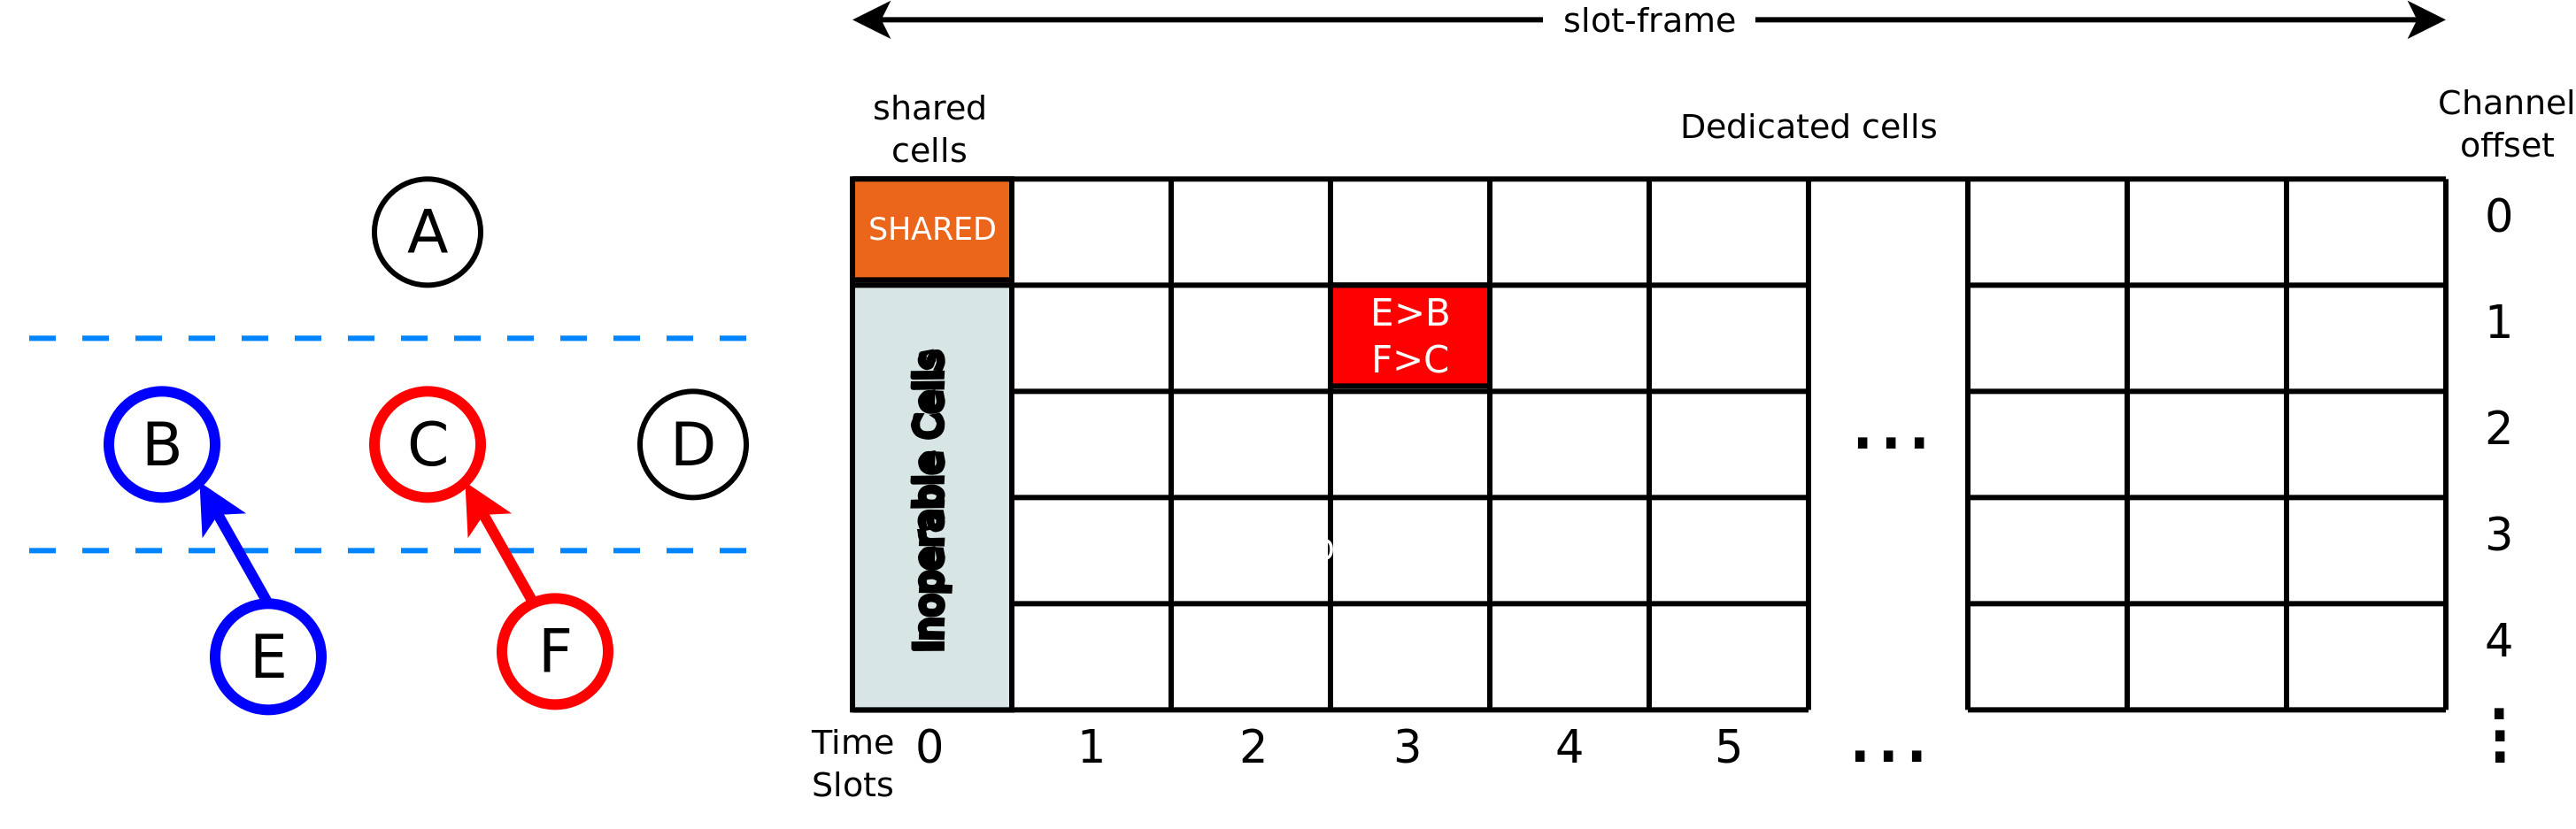
\includegraphics[width=\linewidth]{figures/col2.png}}
  \only<3->{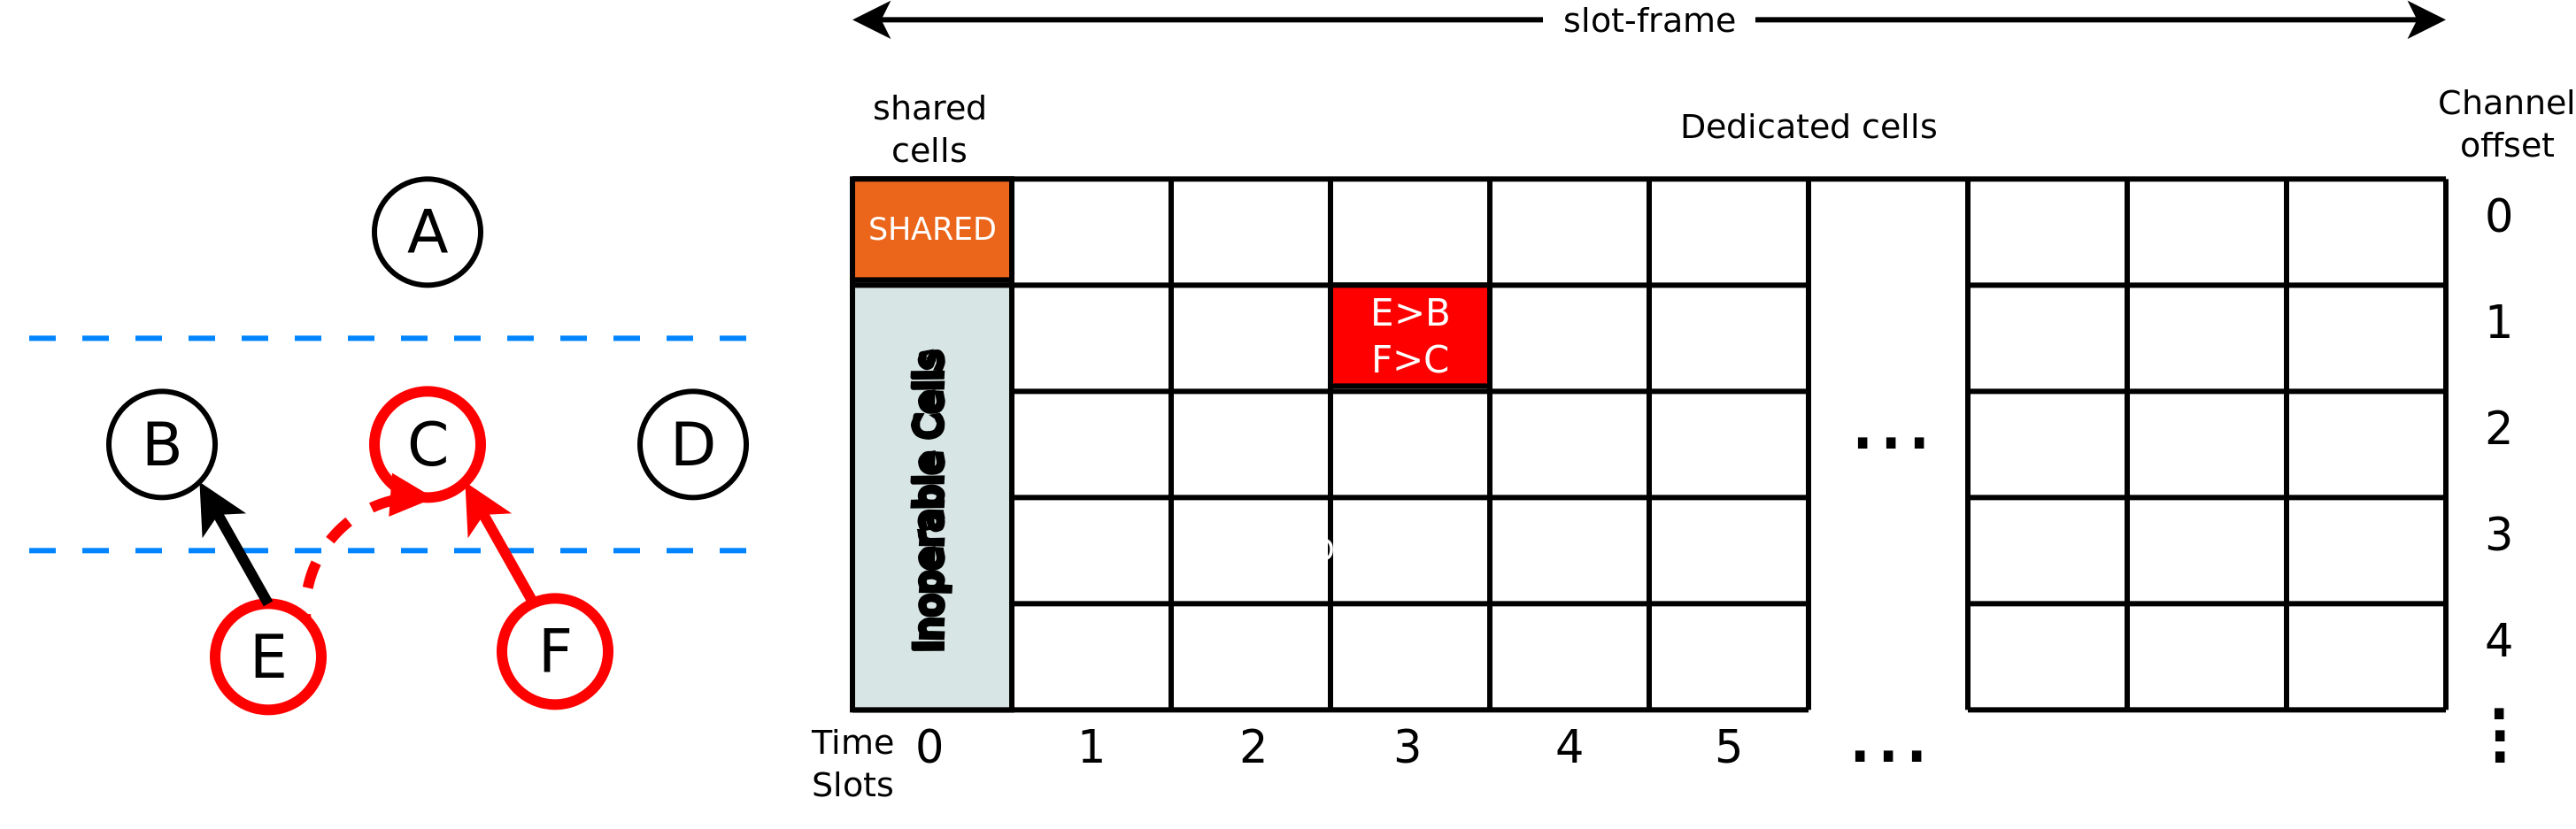
\includegraphics[width=\linewidth]{figures/col3.png}}
  
\end{figure}


\end{frame}
\end{withoutheadline}

%%%%%%%%%%%%%%%%%%%%%%%%%%%%%%%%%%  7   %%%%%%%%%%%%%%%%%%%%%%%%%%%%%%%%



%%%%%%%%%%%%%%%%%%%%%%%%%%%%%%%%%%  8   %%%%%%%%%%%%%%%%%%%%%%%%%%%%%

\begin{withoutheadline}
\begin{frame}{Project Objectives}
\begin{itemize}
\item {Reducing the collisions in TSCH dedicated cells.}
  \item<2-> {Modifying the Cell reserving process without introducing new overhead on the network}
  \item<3-> {Creating a flexible mechanism, compatible with all scheduling functions }

\end{itemize}

\end{frame}
\end{withoutheadline}
